\documentclass[border=10pt]{standalone}
\usepackage{tikz}
\usetikzlibrary{arrows.meta,positioning,decorations.pathmorphing,calc}
\usepackage{amsmath,amssymb}

\begin{document}
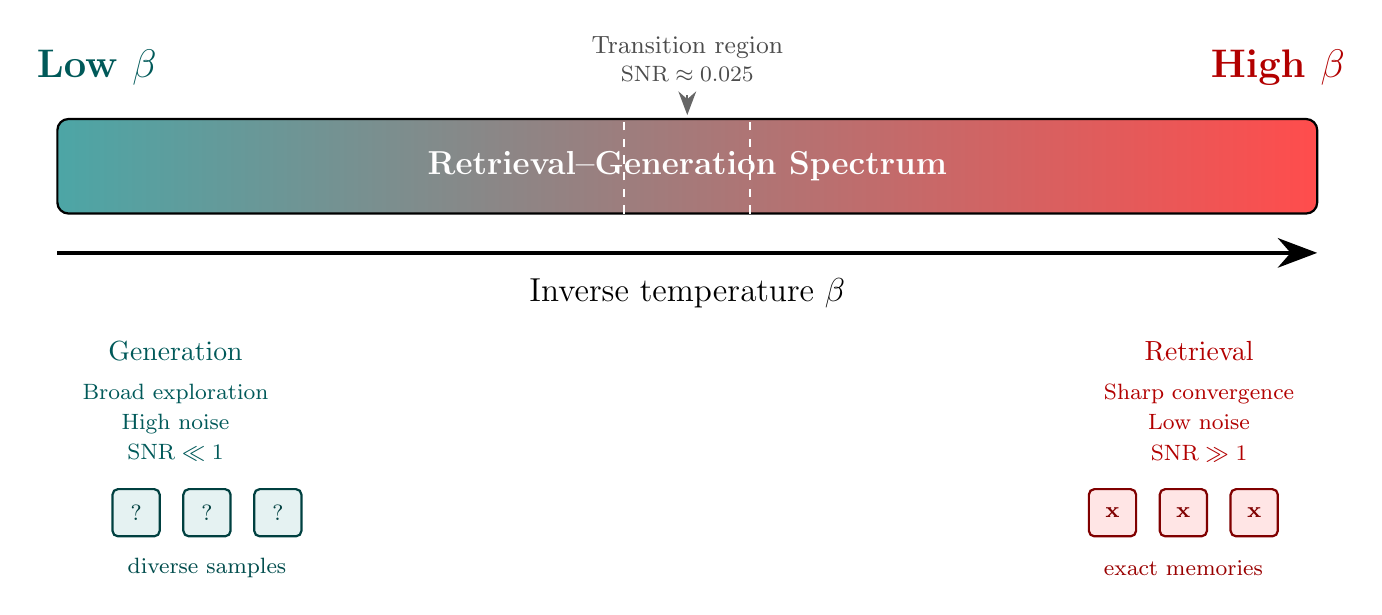
\begin{tikzpicture}

% Main spectrum bar
\def\barlen{16}
\def\barht{1.2}

% Gradient fill from teal (low beta) to red (high beta)
\shade[left color=teal!70, right color=red!70, rounded corners=4pt]
    (0,0) rectangle (\barlen,\barht);

% Border
\draw[thick, rounded corners=4pt] (0,0) rectangle (\barlen,\barht);

% Arrow underneath
\draw[ultra thick, -{Stealth[length=5mm]}] (0,-0.5) -- (\barlen,-0.5);
\node[font=\large, anchor=north] at (\barlen/2, -0.7) {Inverse temperature $\beta$};

% Low beta label (left)
\node[font=\Large\bfseries, teal!70!black, anchor=south] at (0.5, \barht+0.3) {Low $\beta$};
\node[font=\normalsize, teal!70!black, align=center, anchor=north] at (1.5, -1.5) {
    Generation\\[2pt]
    {\footnotesize Broad exploration}\\[-1pt]
    {\footnotesize High noise}\\[-1pt]
    {\footnotesize $\text{SNR} \ll 1$}
};

% High beta label (right)
\node[font=\Large\bfseries, red!70!black, anchor=south] at (\barlen-0.5, \barht+0.3) {High $\beta$};
\node[font=\normalsize, red!70!black, align=center, anchor=north] at (\barlen-1.5, -1.5) {
    Retrieval\\[2pt]
    {\footnotesize Sharp convergence}\\[-1pt]
    {\footnotesize Low noise}\\[-1pt]
    {\footnotesize $\text{SNR} \gg 1$}
};

% Middle region
\node[font=\large\bfseries, white] at (\barlen/2, \barht/2) {Retrieval--Generation Spectrum};

% Transition region marker
\draw[thick, white, dashed] (\barlen*0.45, 0) -- (\barlen*0.45, \barht);
\draw[thick, white, dashed] (\barlen*0.55, 0) -- (\barlen*0.55, \barht);
\node[font=\footnotesize, white, align=center] at (\barlen*0.5, \barht/2+0.05) {};

% Transition annotation
\draw[thick, -{Stealth[length=3mm]}, black!60] (\barlen*0.5, \barht+0.3) -- (\barlen*0.5, \barht+0.05);
\node[font=\small, black!70, anchor=south, align=center] at (\barlen*0.5, \barht+0.35) {
    Transition region\\[-1pt]
    {\footnotesize $\text{SNR} \approx 0.025$}
};

% Example icons - left side (generation = diverse outputs)
\foreach \i in {0,1,2} {
    \node[draw, thick, teal!50!black, rounded corners=2pt, minimum size=0.6cm,
          fill=teal!10] at (1.0+\i*0.9, -3.8) {\footnotesize ?};
}
\node[font=\footnotesize, teal!60!black] at (1.9, -4.5) {diverse samples};

% Example icons - right side (retrieval = matching output)
\foreach \i in {0,1,2} {
    \node[draw, thick, red!50!black, rounded corners=2pt, minimum size=0.6cm,
          fill=red!10] at (\barlen-2.6+\i*0.9, -3.8) {\footnotesize $\mathbf{x}$};
}
\node[font=\footnotesize, red!60!black] at (\barlen-1.7, -4.5) {exact memories};

\end{tikzpicture}
\end{document}
